% !TEX root = ../main.tex

\chapter{Datasets}
\label{ch:datasets}
This Chapter presents the three datasets that have been choosen to be part of this work. The first section, after a small introduction, explains how the choice of these datasets was made. Then, the types of medical images that are used in this work will be described. These types are ones of the most common used. At the end of the second section, a little detour is taken to present the DICOM standard, which is a common standard for medical imaging. Finally in the last section, the three datasets will be presented.


\section{Introduction and choices}
Deep learning models require a lot of data to be efficient (see Section~\ref{sec:deeplearning}). However, in research of deep learning methods in the medical field, data is often scarce. Indeed, lack of publicly available medical data is an issue because of the personal and sensible data of the patients. The data needs to be anonymized before publishing. Today, there exist such publicly available data, provided by the following ressource: the Cancer Imaging Archive (TCIA)~\cite{clark_cancer_2013} is funded by the National Cancer Institute (United States). The data is separated in collections, that have a common disease, the same medical images type (see Section~\ref{sec:medimtype}) or is at the base of a common research goal.

The first part of this work was to choose different datasets to preprocess. Different conferences, like the Medical Image Computing and Computer Assisted Intervention society (MICCAI)\footnote{\url{http://www.miccai.org/}}, the Medical Imaging with Deep Learning (MIDL)\footnote{\url{https://2021.midl.io/}} or the Machine Learning for Healthcare Conference (MLHC)\footnote{\url{https://www.mlforhc.org}} offer many publications in the scope of this work. About 25 publications coming from these conferences were read in detail, but only 5 were retained~\cite{wang_transbts_2021, xie_transferable_2017, ding_accurate_2017, andrearczyk_automatic_2020, wang_residual_2021}. The available datasets of these 5 publications went on a common list. Finally, the work can start with three new datasets choosen from this list. Two of them come directly from TCIA.


\section{Types of medical images}
\label{sec:medimtype}
Depending on the body part to look at, a different type of image or scan can be used. There exist many types of medical images, depending on the hardware, the technology used or the parameters for a same setup. The medical images types are sometimes called the \emph{modality} of the image. Modalities used in this work are:

\vbox{
  \begin{itemize}
    \item Magnetic resonance image (MRI)
    \item Computed tomography (CT) scan
    \item Positron emission tomography (PET) scan
    \item Ultrasound (US) image
  \end{itemize}}
These four modalities will be explained in detail in the following paragraphs. While CT, PET scans and US images come in the datasets presented in this work, the MRI modality comes from previous datasets preprocessed for the \emph{Hydra} framework in the work of~\citet{clement_prostate_2020}.

\subsection{Magnetic resonance image}
The first modality, the \emph{Magnetic resonance image}, produces three-dimensional images from the body, as a stack of 2D images. It uses a strong magnetic field, that will force the protons in the body to align with the field. With a magnetic field that has a frequency dependance, protons will align and dealign as the time passes. This motion of the protons and the energy released during the process is then captured by some sensors, that produce the image. MRI is more often used for soft tissues like muscles, ligments or tendons. For example, MRI is used for the knees, the shoulders or even the brain. To get the image, patients lie on a bed that goes inside a MRI scanner, that has the shape of a closed tunnel, and they stay fixed during the process~\cite{national_institute_of_biomedical_imaging_and_bioengineering_magnetic_nodate}. Figure~\ref{fig:mriprostate} shows a MRI of the prostate.

\subsection{Computed tomography scan}
The second type is the \emph{computed tomography scan}. These scans produce two-dimensional images that can then be stacked to form a full-body image, as for MRI. CT scans use X-rays, that are emitted and go through the body, and are then captured by detectors on the other side. A 2D image is then constructed. CT scans can better see hard tissues, like bones. It can then be used to see bones fractures, but also to image the lungs or the brain. To construct the image, patients lie on a bed that moves slowly through a scanner that has a ring shape. The scanner will emit the X-rays as the patient goes through~\cite{national_institute_of_biomedical_imaging_and_bioengineering_computed_nodate}. Figure~\ref{fig:ctlung} shows a CT scan of the lungs.

\subsection{Positron emission tomography scan}
The third type mentionned is the \emph{positron emission tomography scan}. While the two previous types were non-invasive techniques, the PET is invasive. The patient receives first an intravenous injection of a safe radioactive substance, called the \emph{radiotracer}. The radiotracer is absorbed by the body cells: cells that are diseased will absorb more radiotracer than the healthy ones. This is because the radiotracer accrues in cells that need a lot of glucose. As tumor cells need a significant amount of glucose, it is well absorbed by tumors. By going through a PET scanner, detectors can see which parts have absorbed more of the radiotracer, and can construct 2D images that will be stacked to form a full body three-dimensional image~\cite{cleveland_clinic_pet_nodate}. Figure~\ref{fig:petbrain} shows a PET scan of the brain.

\subsection{Ultrasound image}
Finally, the last type listed above is the \emph{ultrasound images}. This is also a non-invasive technique that uses ultrasound waves emitted from a device named transducer, that is directly touching the skin of the patient. The transducer first projects sound waves within the body, which travel and are then reflected by the different body parts. The transducer listens to the reflected waves, and by measuring the amplitude of the waves and the time they take to reflect, the transducer can compute a 2D image of the tissues and organs. The ultrasound image is then produced in realtime, and can capture the motion of the body parts. This type of image is widely used for several echography, or for breast imaging for example~\cite{national_institute_of_biomedical_imaging_and_bioengineering_ultrasound_nodate}. Figure~\ref{fig:usbreast} shows an ultrasound image of the breast (mammography).

\begin{figure}[t!]
     \centering
     \begin{subfigure}[t]{0.49\textwidth}
        \centering
        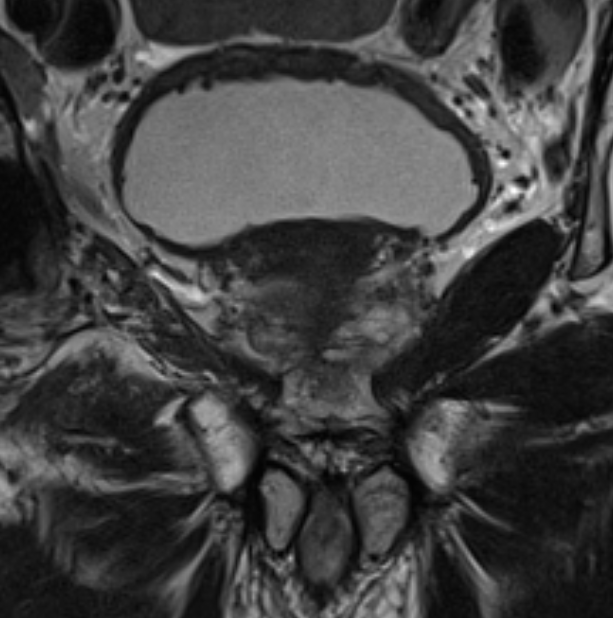
\includegraphics[height=0.25\textheight]{medicalcontext/mriprostate.png}
        \caption[Prostate magnetic resonance image]{Example of a magnetic resonance image of the prostate. This image comes from the PROSTATEx dataset~\cite{armato_prostatex_2018} and has been cropped from the original image.}
        \label{fig:mriprostate}
     \end{subfigure}
     \hfill
     \begin{subfigure}[t]{0.49\textwidth}
        \centering
        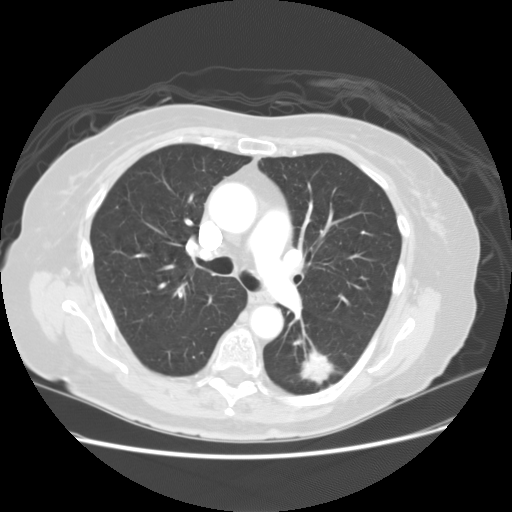
\includegraphics[height=0.25\textheight]{medicalcontext/medimg.png}
        \caption[Lungs computed tomography scan]{Example of a computed tomography scan of the lungs, taken from the LIDC-IDRI dataset~\cite{armato_data_2015}. At the bottom right of the image, a cancerous tumor can be seen, with its typical spider-web-shape.}
        \label{fig:ctlung}
     \end{subfigure}
     \\
     \begin{subfigure}[t]{0.49\textwidth}
        \centering
        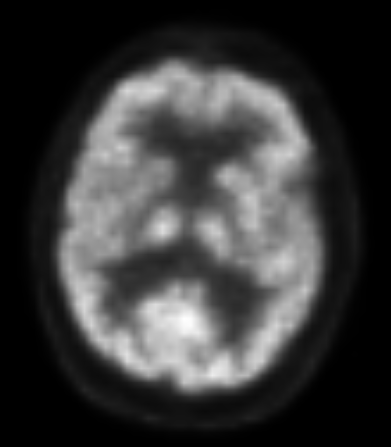
\includegraphics[height=0.25\textheight]{medicalcontext/petbrain.png}
        \caption[Positron emission tomography scan of the brain]{Example of a positron emission tomography scan of the brain from the HNPC dataset~\cite{vallieres_data_2017}.}
        \label{fig:petbrain}
     \end{subfigure}
     \hfill
     \begin{subfigure}[t]{0.49\textwidth}
        \centering
        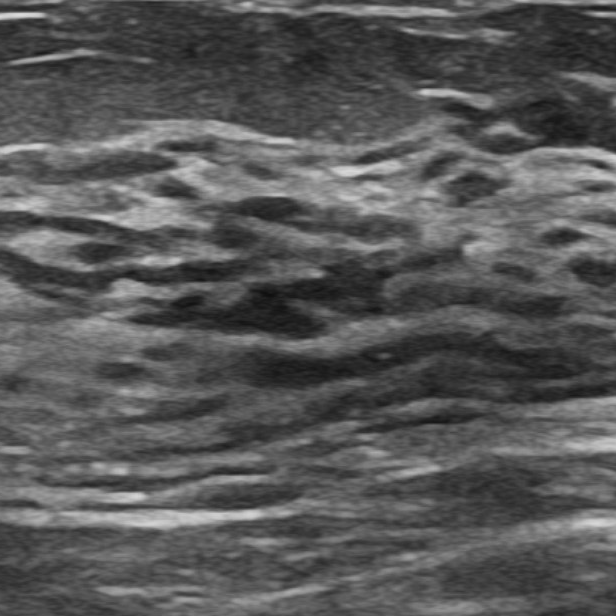
\includegraphics[height=0.25\textheight]{medicalcontext/usbreast.png}
        \caption[Breast ultrasound]{Example of an ultrasound image of the breast, taken from the BUSI dataset~\cite{al-dhabyani_dataset_2020}. This image has been cropped from the original image, to focus on the cancerous tumor.}
        \label{fig:usbreast}
     \end{subfigure}
        \caption[Four different medical images modalities]{Example figure that shows four different modalities of medical images.}
        \label{fig:segmaskimg}
\end{figure}


\section{DICOM standard}
\label{sec:dicom}
Different types of medical images need different hardware, scanners but also the screens on which the image is displayed, or the sensors. All this hardware setup will lead to compatibility problems. Indeed, hospitals around the world have not the exact same hardware to display or create the medical images. When patients go from one hospital to another, images could be displayed differently. To solve this problem, a standardization for medical image is introduced as the \emph{Digital Imaging and Communications in Medicine} (DICOM) standard for medical images and their information. Born in 1993 under the collaboration of the American College of Radiology (ACR) and the National Electrical Manufacturers Association (NEMA), the DICOM standard has revolutionized the medical world, both for doctors and patients. It has enabled advanced medical imaging system, and is one of the most deployed healthcare messaging system. DICOM is the \texttt{ISO~12052:2017} standard~\cite{mildenberger_introduction_2002}.

DICOM files can be recognized by their \texttt{.dcm} file extension. The structure of a \mbox{DICOM} file can be represented as a dictionary structure, each entry being a \mbox{key-value} pair. Keys are called \emph{DICOM tags} and are tuples of two hexadecimal numbers, uniquely identified, which correspond to a certain value. A tool that explains and describes all DICOM tags of all type of images is available at the DICOM standard browser\footnote{\url{https://dicom.innolitics.com/ciods}}. These hundred of different tags contain all medical information: from the patient information, to the size of the image, to the type of image, to some numeric identifiers, to settings of the scanner who takes the image. Each DICOM file contains all these tags but also one or more 2D images (slices), stored in a specific DICOM tag, named \texttt{Pixel Data}. Figure~\ref{fig:dicom} shows an example of DICOM tags available in a CT scan.

To solve the compatibility problems mentioned above, DICOM provides some information in its tags. For example, it provides slope and intercept values to rescale the image (tags \texttt{(0028,1052)} and \texttt{(0028,1053)}). Additional information like the pixel spacing (tag \texttt{(0028,0030)}) or bits allocated (tag \texttt{(0028,0100)}) are also useful to normalize images from a dataset. Section \ref{sec:imgconversion} shows more technical details to convert medical images.

\begin{figure}[t!]
  \centering
  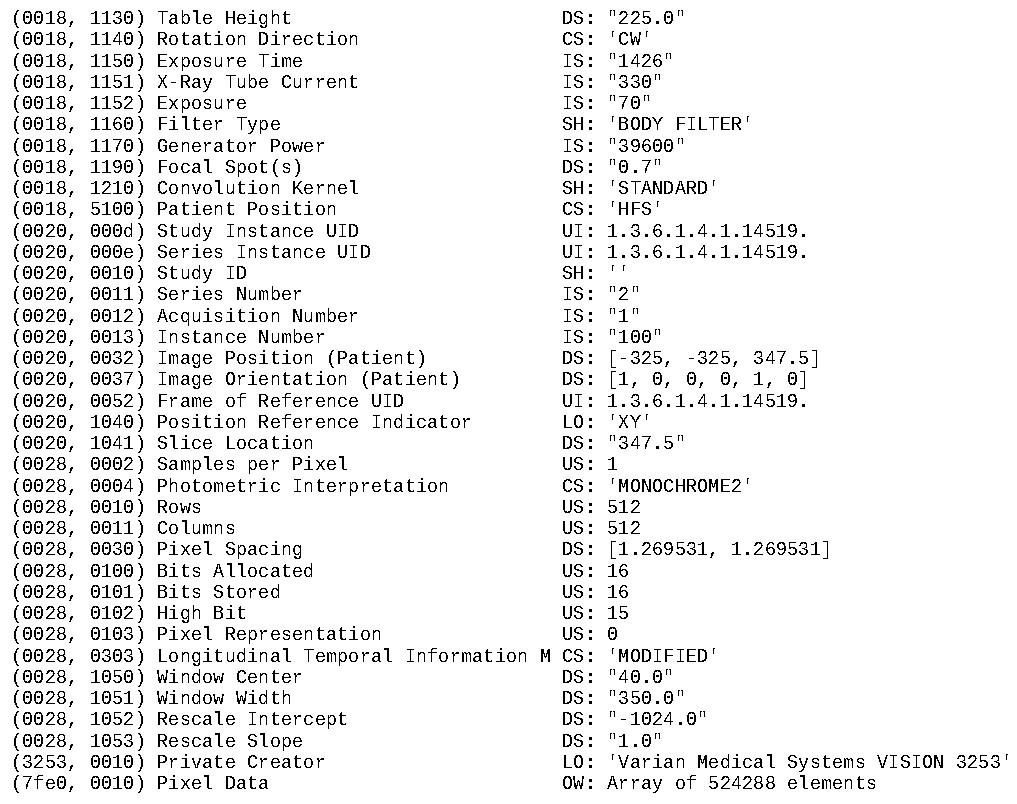
\includegraphics[width=\textwidth]{datasets/dicom.pdf}
  \caption[DICOM tags example]{DICOM file content example for a CT scan. On the left, DICOM tags which are tuples of two hexadecimal numbers, have an associated name to be readable by humans. On the right, the value of each DICOM tag is displayed. The \texttt{UID} tags values have been cut for readability.}
  \label{fig:dicom}
\end{figure}


\section{Lung Image Database Consortium image collection}
The first dataset that will be used in this work is the Lung Image Database Consortium image collection (LIDC-IDRI) dataset~\cite{armato_data_2015}. This dataset is the result of the collaboration of seven academic centers and eight medical imaging companies, under the initiation of the \emph{National Cancer Institute} (NCI), with the help of the \emph{Food and Drug Administration} (FDA) (United States). The goal of this collaboration and this dataset is "to develop, train and evaluate computer aided-diagnosis methods for lung cancer detection and diagnosis"~\cite{armato_lung_2011}.

The dataset contains three different types of scans: computed tomography (CT), digital radiography (DX) and computed radiography (CR) scans of the lungs. These scans cover about 1000 different patients, for a total of more than 240'000 images. All images in the dataset are in the DICOM format. In the LIDC-IDRI dataset, four radiologists have participated together to analyze and mark the whole set of CT scans. \citet{xie_transferable_2017} and \citet{ding_accurate_2017} have used this dataset for a detection task, while in this work it is used for a localization and a segmentation task (see Section~\ref{sec:lidcpreproc}).

The work of analysing this dataset has been separated in two different phases. During the first phase, the radiologists read all the CT scans in a blind manner, i.e. the radiologists have never seen the images before, and they do not know anything about the past history of the patients. Each radiologist was on his own, with no additional information, and had to mark the lesions and class them in three different categories:

\vbox{
  \begin{enumerate}
    \item Nodules >= 3 mm diameter
    \item Nodules < 3 mm diameter
    \item Non-Nodules >= 3 mm diameter
  \end{enumerate}}

For the first category, the radiologists drew the contour of this type of nodule in each slice of CT scan where the nodule appeared. Then, they were asked to subjectively give their opinion about some characteristics related to the nodule, for example the difficulty to detect the nodule, its internal structure, how well its margins are defined, or its malignancy. All characteristics are given in a scale between 1 and 5.

For the last two categories, the radiologists just gave the three-dimensional center of mass of these (non-)nodules.

\newpage
During the second phase, the results of the first phase were complied and send back to the four radiologists. They then read the marking work of the other radiologists. Finally, with the help of the four diagnoses, they were been asked to make a final decision about the marking and the characteristics.

All diagnoses, characteristics and annotations of the radiologists are stored in XML files. There is one XML file per CT series. An example of XML file for a nodule of the first category (Nodules >= 3 mm) is showed in the Listing~\ref{lst:lidcxml}. This example contains a nodule ID, the characteristics mentioned before, and the contour of the nodule, which is contained in the tag named \texttt{roi} (region of interest). The contour contains all the $x$ and $y$ coordinates of the points that make the contour of the nodule, and the universal identifier (UID) of the corresponding slice.

\lstinputlisting[float=t!, language=XML, caption={XML content example for a nodule >= 3 mm of the LIDC-IDRI dataset~\cite{armato_data_2015}. There is a nodule ID, some characteristics and a \texttt{roi} (region of interest) tag that contains the contour points $(x,y)$ of the nodule. The \texttt{imageSOP\_UID} tag has been left out for readability.}, label=lst:lidcxml, captionpos=b]{figures/datasets/lidcxml.xml}

\newpage
\section{Head-Neck-PET-CT dataset}
The second dataset that will be used in this work is the Head-Neck-PET-CT (HNPC) dataset~\cite{vallieres_data_2017}. It is a compilation of images, diagnoses and other medical information that are coming from four different institutions in Québec, Canada. 92 patients are coming from the \emph{Hôpital Général Juif} (HGJ) in Montréal, 102 from the \emph{Centre Hospitalier Universitaire de Sherbrooke} (CHUS), 41 patients from the \emph{Hôpital Maisonneuve-Rosemont} (HMR), and finally 65 from the \emph{Centre hospitalier de l’Université de Montréal} (CHUM).

The dataset contains computed tomography (CT) and positron emission tomography (PET) scans of the head, including the brain, to the neck. Both images types are given in the DICOM format. The HNPC dataset contains 300 different patients, that all have histologically proven head and neck cancer. The dataset contains a total of about 120'000 images. This patients data was used first in the work of \citet{vallieres_radiomics_2017}, that has been the trigger of the creation and compilation of the HNPC dataset.

The HNPC dataset contains, for each patient, several series. For each CT and PET scans series mentionned before, there is a corresponding radiotherapy structure set (RTStruct) series, that is a single DICOM file containing the contour points for several regions of interest (ROI) inside a DICOM tag. To illustrate, Figure~\ref{fig:hnpc_structset} shows a part of the \texttt{structure set ROI} DICOM tag, that contains ROI names and their correponding ROI number used further in the RTStruct, as a reference. The RTStruct file contains then, for each slice of its corresponding images series, the contour points of the ROIs and also a universal identifier that uniquely identifies the corresponding slice. These RTStruct series are the result of the work of radiologists coming from the four different institutions, that draw the contour of the ROIs, including tumors. The dataset contains also two other series named radiotherapy plan (RTPlan) and radiotherapy dose (RTDose). These two series contain more medical information about the patients, such as the planning of the therapy or the scheduling for the doses given to the patients.

With the HNPC dataset, two excel files are attached. The first of the two excel files is called \texttt{INFO\_clinical\_HN.xlsx} and contains textual medical information about all the patients, including for example the stage of the cancer, its primary location, the time of the diagnosis or the length of the treatment. In the second excel file, named \texttt{INFO\_GTVcontours\_HN.xlsx}, the gross tumor volume (GTV) names are listed under the same name as they appear in the RTStruct, as ROI name (see the DICOM tags \texttt{(3006,0026)} of the Figure~\ref{fig:hnpc_structset}).

\begin{figure}[t!]
  \centering
  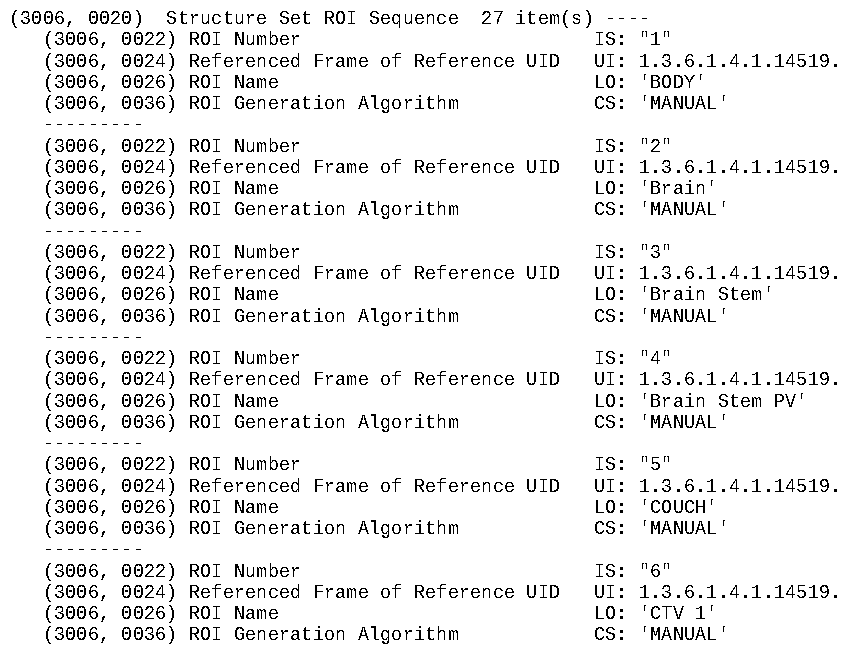
\includegraphics[width=\textwidth]{figures/datasets/hn_structsetroi.pdf}
  \caption[RTStruct DICOM content]{DICOM content example for an RTStruct series of the HNPC dataset~\cite{vallieres_data_2017}. DICOM tags can be seen on the left as tuples of two hexadecimal numbers, and their corresponding value can be seen on the right. The \texttt{UID} tags values have been cut for a better readability of the image.}
  \label{fig:hnpc_structset}
\end{figure}

\newpage
\section{Breast Ultrasound Images dataset}
The third and last dataset used in this work is the Breast Ultrasound Images (BUSI) dataset~\cite{al-dhabyani_dataset_2020}. This dataset is a collection of ultrasound images from the breast. The images were all collected in 2018, and they come from 600 different female patients, aged from 25 to 75. Originally, 1100 ultrasound images were collected at the \emph{Baheya hospital} in Egypt, under the DICOM format. Before constructing the dataset, radiologists have marked and reviewed annotations in the images.

The BUSI dataset contains, after reduction, a total of 780 ultrasound images, cropped and converted into the PNG format. The ground truth images, i.e. the segmentation masks, are given along the original images. These segmentation masks have been created by the radiologists over a year of work. For some images, there are more than one segmentation mask, if there is more than one tumor. The breast ultrasound images are separated in three categories: normal, benign and malignant. Each of these categories is a complete folder given in the dataset, containing images and their segmentation masks.
